% LaTex for Computer Architecture final project
\documentclass[conference]{IEEEtran}
\IEEEoverridecommandlockouts
\usepackage{cite}
\usepackage{amsmath,amssymb,amsfonts}
\usepackage{algorithmic}
\usepackage{graphicx}
\usepackage{textcomp}
\usepackage{xcolor}
\usepackage{hyperref}
\def\BibTeX{{\rm B\kern-.05em{\sc i\kern-.025em b}\kern-.08em
    T\kern-.1667em\lower.7ex\hbox{E}\kern-.125emX}}
\begin{document}

\title{Single Cycle Datapath Processor using MIPS\\
}

\author{\IEEEauthorblockN{Piero Morales}
\IEEEauthorblockA{\textit{Computer Science University Student} \\
\textit{University of Engineering and Technology}\\
Lima, Peru \\
piero.morales@utec.edu.pe}
\and
\IEEEauthorblockN{Angel Motta}
\IEEEauthorblockA{\textit{Computer Science University Student} \\
	\textit{University of Engineering and Technology}\\
	Lima, Peru \\
	angel.motta@utec.edu.pe}
}

\maketitle

\begin{abstract}
Two undergraduates implemented a 32 bits pathline based on RISC MIPS for a computer architecture course. This datapath support instructions R-type, I-type and J-type. This included designing the architecture in Verilog, developing test bench modules for the implementation.
\end{abstract}

\begin{IEEEkeywords}
Computer architecture, risc, verilog, processor, big endgian, microprocessor without interlocked pipeline stages
\end{IEEEkeywords}

\section{Introduction}	%I. Introduction
The form, design, and implementation of CPUs have changed over the course of their history, but their
fundamental operation remains almost unchanged. The CPU has become the nerve center of any computer,
from mobile devices to supercomputers. From the beginning	of computer era scientists have tried to improve
processor performance not only increasing the number of transistors, but also by improving the instructions
that the processor executes. A major change that happened for CPUs is the paradigm from a single core to multi core that increased signifcantly its performance. In this way, Moore's law, that until this moment had traced the future of processors,
is discarded.
\section{Methodology}	%II. Methodology

For this project we use a Hardware Description Language (HDL) to design and simulate our
processor and all its components related. The datapath was coded in Verilog. We choose Verilog \cite{b2} as HDL because is widely used in the industry and it was simulated and tested using test bench modules.

The goal of this project is achieve a better understanding of MIPS single-cycle and implement it with focussing in the basic operations with integers, covering R-type, I-type and J-type instructions for 32 bits MIPS ISA:

\begin{table}[htbp]
\caption{R Type} %R Type
\begin{center}
\begin{tabular}{|c|c|c|}
\hline
\multicolumn{3}{|c|}{\textbf{Instructions}} \\
%\cline{2-4} 
\hline
ADD&Subtraction&AND  \\
&(SUB)&\\
\hline
NOR&OR&Set Less Than\\
&&(SLT)\\
\hline
Jump Register&& \\
(JR)&&\\
\hline
\end{tabular}
\label{tab_rtype}
\end{center}
\end{table}

\begin{table}[htbp]
\caption{I Type} %I Type
\begin{center}
\begin{tabular}{|c|c|c|}
\hline
\multicolumn{3}{|c|}{\textbf{Instructions}} \\
%\cline{2-4} 
\hline
Add Immediate&Subtraction Inmediate & AND Inmediate \\
(ADDI) &(SUBI) & (ANDI) \\
\hline
OR Immediate&Set Less Than Immediate&  Store Byte \\
(ORI)&(SLTI)&(SB) \\
\hline
Store Halfword&Store Word&Load Byte \\
(SH)&(SW)&(LB)\\
\hline
Load Halfword&Load Word&Load Upper\\
(LH)&(LW)&Immediate (LUI)\\
\hline
Branch On Equal&Branch On Not Equal&Branch On Greater \\
(BEQ)&(BNEQ)&than equal zero (BGEZ)  \\
\hline
\end{tabular}
\label{tab_itype}
\end{center}
\end{table}

\begin{table}[htbp]
\caption{J Type} %J Type
\begin{center}
\begin{tabular}{|c|c|c|}
\hline
\multicolumn{3}{|c|}{\textbf{Instructions}} \\
%\cline{2-4} 
\hline
Jump&Jump and Link&\\
(J) &(JAL)&----\\
\hline
\end{tabular}
\label{tab_itype}
\end{center}
\end{table}
\subsection{Datapath}
To achieve the goal of supporting all instructions listed before we need to implement the following components:

\begin{itemize}
\item Aritmetic Logic Unit (ALU), one of the core componentes of the processor who make the operations of addition, subtraction, comparation between two numbers, logic AND, logic OR, logic NOR.
\item Instruction Memory, stores all the instructions to be read and executed according to the address selected.
\item PC Counter, a register to hold the address of the current instruction being executed.
\item Register File, space that stores 32 registers for MIPS ISA, each one of 32 bits.
\item Data Memory, stores the data to support load and stores instructions.
\item Multiplexor 2 to 1, determine which of the 2 inputs input select, based on a selector signal i.e. in the selection between the PC Counter, the branch or the jump.
\item Adder, execute PC + 4 to link the following instruction, also is used for the offset to cover the branch instruction.
\item Shift Left 2 and 16, to be used to calculate the offset for the branch and load a number 
up to 32 bits respectively.
\item Sign extend, used to extend the most significant bit of the number.
\item and the control component for support all the instructions deciding which signal activate 
depending on the type of instruction and the operation.
\end{itemize}

The structure of the datapath including all the components:
\begin{figure}[h]
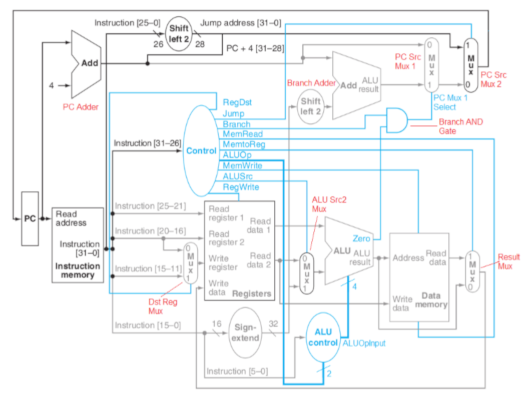
\includegraphics[scale=2]{datapath.png}
\caption{Datapath.}
\end{figure}
%\begin{figure*}[htbp]
%\centerline{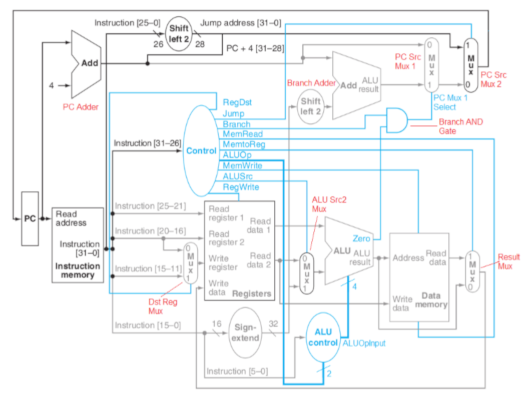
\includegraphics[scale=0.25]{datapath.png}}
%\caption{Datapath.}
%\label{fig_data}
%\end{figure*}

\subsection{Verilog}
The implementation in Verilog is in a single file called \verb$Datapath.v$ where is coded the instruction set architecture. Three differents files called \verb$instruction.txt$ are used to test and validate the correct functionality of the implementation along with a file called \verb$Test_datapath.v$
In total the implementation is composed of the following 5 files:

\begin{table}[htbp]
\begin{center}
\begin{tabular}{c c}
\verb$Datapath.v$&\verb$(implementation)$\\
\verb$Test_datapath.v$&\verb$(testing module)$\\
\verb$instruction.txt$&\verb$(for R-type)$\\
\verb$instruction.txt$&\verb$(for I-type)$\\
\verb$instruction.txt$&\verb$(for J-type)$\\
\end{tabular}
\end{center}
\end{table}

\section{Experimental Setup} %III Experimental Setup
The implementation of the datapath has the following setup
\subsection{Instructions and opcodes}
The opcodes used in the implementation are shown in the Table IV
\begin{table}[htbp]
	\caption{Opcode MIPS} %Testbench 1
	\begin{center}
		\begin{tabular}{|c|c|c|c|}
			%\cline{2-4} 
			\hline
			N&TYPE&OPCODE&OPERATION\\
			\hline
			1&ADD&000000&add \$s0,\$t0,\$t1\\
			\hline
			2&SUB&000001&add \$s1,\$t2,\$t3\\
			\hline
			3&AND&000010&and \$s2,\$t4,\$t5\\
			\hline
			4&NOR&000011&nor \$s3,\$t6,\$t7\\
			\hline
			5&OR&000100&or \$s4,\$t8,\$t9\\
			\hline
			6&SLT&000101&slt \$s5,\$t0,\$t1\\
			\hline
			7&ADDI&000110&addi \$s6,\$t2,45\\
			\hline
			8&SUBI&000111&subi \$s7,\$t3,37\\
			\hline
			9&ANDI&001000&andi \$s0,\$t4,66\\
			\hline
			10&ORI&001001&ori \$s1,\$t5,89\\
			\hline
			11&SLTI&001010&slti \$s2,\$t6,65535\\
			\hline
			12&LB&001011&lb \$s3,33,(\$zero)\\
			\hline
			13&LH&001100&lh \$s4,65(\$zero)\\
			\hline
			14&LW&001101&lw \$s5,48(\$zero)\\
			\hline
			15&LUI&001110&lui \$s6,346\\
			\hline
			16&MUL&001111&mul \$s2,\$s0,\$s1\\
			\hline
			17&SB&010000&sb \$s7,24(\$zero)\\
			\hline
			18&SH&010001&sh \$s0,73,(\$zero)\\
			\hline
			19&SW&010010&sw \$s1,91,(\$zero)\\
			\hline
			20&BEQ&010011&beq \$t0,\$t1,1\\
			\hline
			21&BNEQ&010100&bneq \$t2,\$t3,1\\
			\hline
			22&BGEZ&010101&bgez \$t4,10\\
			\hline
			23&J&010110&j 12\\
			\hline
			24&JAL&010111&jal 15\\
			\hline
			25&JR&011000&jr \$ra\\
			\hline
		\end{tabular}
	\label{tab_opcode}
\end{center}
\end{table}

\subsection{Register File}
32 registers, each one of 32 bits.
\subsection{Instruction memory}
Size: 256 bytes
\subsection{Data memory}
Size: 256 bytes\\
\subsection{Data memory}
Size: 256 bytes\\
\subsection{Testbench}
Each test bench is using 5 nanoseconds as a positive clock signal and negative clock signal which give us 10 nanoseconds in total per clock cycle.

\begin{table}[htbp]
\caption{Testbench 1} %Testbench 1
\begin{tabular}{|c|c|c|}
\hline
\multicolumn{3}{|c|}{\textbf{Instructions}} \\
%\cline{2-4} 
\hline
ADD&Subtraction (SUB)&AND  \\
\hline
NOR&OR&Set Less Than (SLT) \\
\hline
Add Immediate&Subtraction Inmediate & AND Inmediate \\
(ADDI) &(SUBI) & (ANDI) \\
\hline
OR Immediate&Set Less Than Immediate&  \\
(ORI)&(SLTI)&  \\
\hline
\end{tabular}
\label{tab_test1}
\end{table}

\begin{table}[t]
\caption{Testbench 2} %Testbench 2
\begin{center}
\begin{tabular}{|c|c|c|}
\hline
\multicolumn{3}{|c|}{\textbf{Instructions}} \\
%\cline{2-4} 
\hline
Store Byte&Store Halfword&Store Word\\
(SB)&(SH)&(SW)  \\
\hline
Load Byte&Load Halfword&Load Word\\
(LB)&(LH)&(LW) \\
\hline
Load Upper Inmediate&&\\
(LUI)&& \\
\hline
\end{tabular}
\label{tab_test2}
\end{center}
\end{table}

\begin{table}[htbp]
\caption{Testbench 3} %Testbench 3
\begin{center}
\begin{tabular}{|c|c|c|}
\hline
\multicolumn{3}{|c|}{\textbf{Instructions}} \\
%\cline{2-4} 
\hline
Branch On Equal&Branch On Not Equal&Branch On Greater \\
(BEQ)&(BNEQ)&than equal zero (BGEZ)  \\
\hline
Jump&Jump and Link&Jump Register\\
(J)&(JAL)&(JR) \\
\hline
\multicolumn{3}{l}{Since we need to simulate the branch and the jumps between the} \\
\multicolumn{3}{l}{instructions additional instructions were added i.e. ADDI and  SUB}\\
\end{tabular}
\label{tab_test3}
\end{center}
\end{table}

To get a real aproach of the use of the processor we will run the following C code.
\begin{figure}[h]
\begin{center}
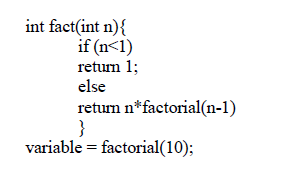
\includegraphics[scale=0.8]{factorial_c.png}
\caption{Factorial function - C code.}
\label{fact_c}
\end{center}
\end{figure}

The translation into MIPS instructions it would be as follow:
\begin{figure}[h]
\begin{center}
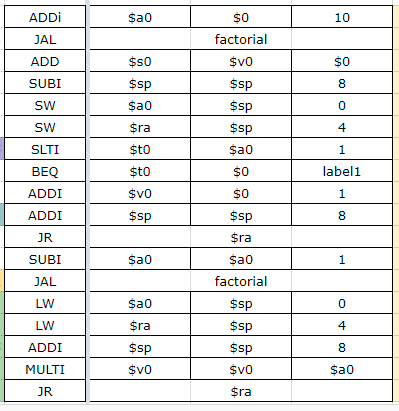
\includegraphics[scale=0.55]{factorial_mips.png}
\caption{Factorial function - MIPS.}
\label{fact_mips}
\end{center}
\end{figure}
 
As we can use the factorial function will use most of the intructions implemented and the recursivity
technique, this will be our test bench 4.

To calculate the CPU time \cite{b5} (time processing) for each test bench we use the following formula:
\[Time = PI * CPI * Time per Clock Cycle\] 

where PI is Program Instructions and CPI is Clock Cycles per instruction. 

\begin{table}[h]
\caption{Clock cycles} %Clock cycles
\begin{center}
\begin{tabular}{|c|c|c|c|c|}
\hline
&Total&Total executed&Clock&CPU Time\\
&instructions&instructions&Cycles&(Nanoseconds)\\
&&(Expected)&&\\
\hline
Test bench 1&11&11&11&220\\
\hline
Test bench 2&7&7&7&140\\
\hline
Test bench 3&22&17&17&340\\
\hline
Test bench 4&18&131&131&2620\\
\hline
\end{tabular}
\label{tab_test3}
\end{center}
\end{table}

%EVALUATION SECTION
\section{Evaluation}
We executed the test bench 1, 2, 3 and 4, these were the results:

\begin{figure}[h]
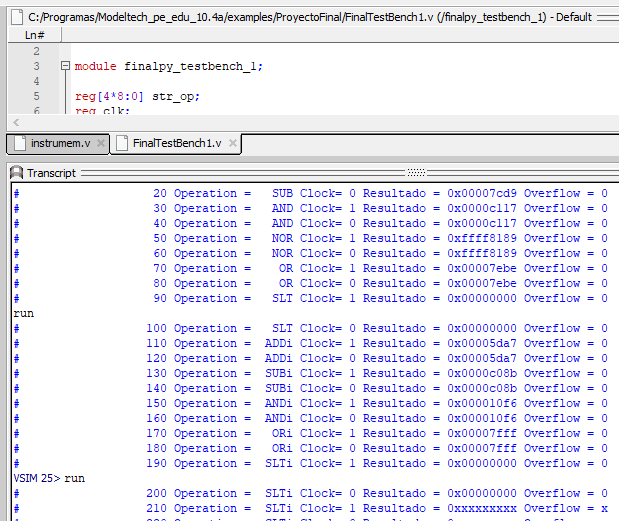
\includegraphics[scale=0.41]{ModelSim_testbench1_clock_cycles.png}
\caption{Execution results for test bench 1.}
\label{result1}
\end{figure}

We ran the test bench in intervals of 100 nanoseconds as we can see in Fig. 5. \label{result1}. For the 
test bench 1 we get 100 nanoseconds + 100 nanoseconds + 20 nanoseconds with in total 
give us 220 nanoseconds.

We apply the same procedure to the test bench 2  \label{result3}, Fig. 8. and the result was
100 nanoseconds + 40 nanoseconds = 140 nanoseconds.

In test bench 3, Fig. 9., we got 100 nanoseconds + 100 nanoseconds + 100 nanoseconds 
+ 40 nanoseconds with th total of 340 nanoseconds.

And finally for the test bench 4, Fig. 6, we use intervals of 500 nanoseconds since the execution
is elevated, we get 2610 nanoseconds in total also the output of the factorial of 10 was 
0x003750f00 which in decimal notation correspond to 3628800.

\begin{figure}[h]
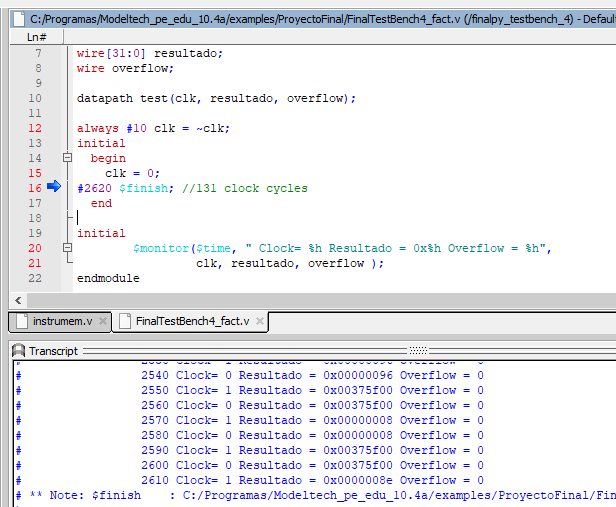
\includegraphics[scale=0.5]{ModelSim_factorial4_clock_cycles.png}
\caption{Execution results of the test bench for the factorial.}
\label{result_factorial}
\end{figure}

\begin{figure}[h]
\begin{center}
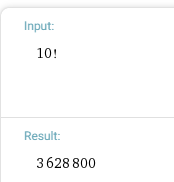
\includegraphics[scale=0.7]{factorial_10.png}
\caption{Wolfram Alpha - Factorial of 10. \cite{b6}}
\label{result_factorial}
\end{center}
\end{figure}

\begin{figure}[h]
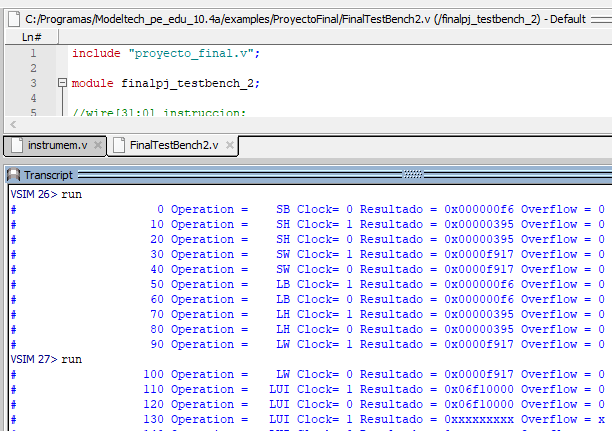
\includegraphics[scale=0.5]{ModelSim_testbench2_clock_cycles.png}
\caption{Execution results for test bench 2.}
\label{result2}
\end{figure}

\begin{figure}[h]
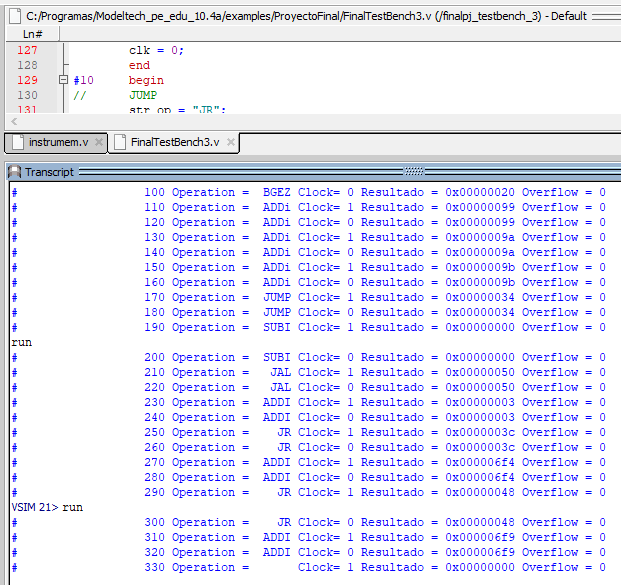
\includegraphics[scale=0.5]{ModelSim_testbench3_clock_cycles.png}
\caption{Execution results for test bench 3.}
\label{result3}
\end{figure}

Comparing the results of Fig. 5., Fig. 8. and Fig. 9. with the Table VIII we get the same amount
of clock cycles and the time for each file, also the results of the instructions are as we expected.
 
%CONCLUSION SECTION
\section{Conclusion}
\begin{itemize}
\item A team of 2 undergraduates designed and implemented and tested a 32-bits MIPS processor. The implementation was completed as part of an academic semester-long Computer Architecture course.
\item This implementation of single-cycle datapath is a close replica of the original in the early days of RISC architecture. Nowadays this approach show limitations of performance due to the execution of 1 instruction per cycle and this implementation is not considering pipeline technique to improve the performance.
\item The implementation successfully passed all tests bench including a factorial program which used many components of the architecture.
\end{itemize}
%COMMENTS SECTION
\section{Comments}
\begin{itemize}
\item When we are simulating our component in ModelSim no warnings must appear when the 
simulation starts, otherwise there was some error or unexpected behaviour. One common 
issue is referring a wire or register as an input or output of a module with diferent length.
\item In ModelSim is the identifier is not declare verilog assume is a wire.
\item The verilog compiler doesn't warn you when a module  instantiation does not exists until you simulate it
\item One common problem is asume the execution of the code in the components of the datapth will be sequential, 
that is not correct since we have the always @ block and that could be executed in the upper sign of the clock 
or the lower sign.
\item For those who are used to the conditional statements of the programming languages it is a little difficult at the 
beginning use verilog, because at the digital circuit level there we only have and, or, xor and all the gates.
\item To find the errors in the testing fase we can navigate in the windows objects in ModelSim throught the modules
to find the issue.
\end{itemize}

\begin{thebibliography}{00}
\bibitem{b1} MIPS.com. (2016). MIPS® Architecture for Programmers Volume II-A: The MIPS32® Instruction Set Manual. [online] Available at: \url{https://s3-eu-west-1.amazonaws.com/downloads-mips/documents/MD00086-2B-MIPS32BIS-AFP-6.06.pdf} [Accessed 27 Nov. 2018].
\bibitem{b2} IEEE Standard for Verilog Hardware Description Language. IEEE Standard 1364-2005 (Revision of IEEE Standard 1364-2001). \url{http://dx.doi.org/10.1109/IEEESTD.2006.99495}, 2006. Last access 26 November 2018.
\bibitem{b3} Mentor.com. (2018). ModelSim PE Student Edition. [online] Available at: \url{https://www.mentor.com/company/higher_ed/modelsim-student-edition} [Accessed 27 Nov. 2018].
\bibitem{b4} Ashenden, P. (2008). Digital Design: An Embedded Systems Approach Using Verilog. Burlington, MA: Elsevier Science, pp.22,23.
\bibitem{b5} Patterson, D., Hennessy, J. and Alexander, P. (2012). Computer organization and design. 4th ed. Waltham, Mass: Morgan Kaufmann, pp.35.
\bibitem{b6} Wolframalpha.com (2018). Wolfram|Alpha: Making the world’s knowledge computable. [online] Wolframalpha.com. \url{Available at: https://www.wolframalpha.com/input/?i=factorial+10} [Accessed 28 Nov. 2018].
\end{thebibliography}
\vspace{12pt}

\end{document}
